% Metódy inžinierskej práce

\documentclass[10pt,oneside,slovak,a4paper]{article}

\usepackage{float}
\usepackage[slovak]{babel}
\usepackage[IL2]{fontenc} 
\usepackage[utf8]{inputenc}
\usepackage{graphicx}
\usepackage{url} 
\usepackage{hyperref} 
\usepackage{cite}
\usepackage{times}

\usepackage{subcaption}
\usepackage{caption}

%\pagestyle{headings}

\title{Softvéry na detekciu potencionálnych rizík 
implementované v automobiloch\thanks{Semestrálny projekt v predmete Metódy inžinierskej práce, ak. rok 2021/22, vedenie: PhD. Ing. Fedor Lehocki  }} 

\author{Michal Januška\\[2pt]
	{\small Slovenská technická univerzita v Bratislave}\\
	{\small Fakulta informatiky a informačných technológií}\\
	{\small \texttt{xjanuskam@stuba.sk}}
	}

\date{\small 5.10. 2021}



\begin{document}

\maketitle

\begin{abstract}
Žijeme v dobe, kde už je vlastníctvo automobilu komoditou. Tieto stroje sú nám veľkou výpomocou či už pri výkone práce alebo pri voľnočasových aktivitách. Aj keď sa na prvý pohľad môže zdať, že automobily so sebou prinášajú samé výhody, nastávajú aj také situácie kedy sa toto vozidlo môže vymknúť kontrole vodiča a môže dôjsť  k veľmi nebezpečným situáciam alebo až k smrteľným nehodám. V takýchto situáciach nastupujú rôzne zabudované softvéry, ktoré majú za úlohu včas detekovať hroziace riziko a vykonať všetko pre jeho zabránenie s dôrazom na čo najmenšie ohrozenie posádky automobilu ale aj vonkajšieho prostredia. Tieto softvéry fungujú na báze umelej inteligencie a machine learningu. V tejto práci sa venujem predstaveniu týchto softvérov z rôznych aspektov a ich funkcionalite ktorá spočíva v modelovaní postupov riešení pri rizikových situáciach.
\end{abstract}



\section{Úvod}\label{uvod}

Zameranie tejto práce je pomerne široké, preto sa ho budem snažiť interpretovať čo najjednoduchšie a najstručnejšie. Hneď v sekcii~\ref{problematika} si predstavíme riziká ktoré môžu nastať pri vedení automobilu alebo aj pri automobile ktorý nie je práve v pohybe. V nasledujúcej sekcii~\ref{predstavenie} si predstavíme softvéry a pomocné komponenty ktoré majú za úlohu sa s týmito situáciami vysporiadať a urobíme ich podrobný rozbor. Niektoré z týchto komponentov ešte momentálne nie je implementovaných v bežných automobiloch, ale vývojári sa ich snažia dokončiť čo najrýchlejšie a následne vyslať na trh. Budeme sa zaoberať vytváraním modelov daných situácií a ukážeme si ich priebeh od začiatku až do konca. V tejto práci nebudem poukazovať len na výhody týchto softvérov a zariadení, ale budem uvádzať aj nevýhody a ich potencionálne odstránenie. Rozbor jednotlivých softvérov a komponentov bude obohatený o rôzne grafy a vývojové diagramy, pre lepšie pochopenie danej problematiky. Celá práca bude zhrnutá v sekcii~\ref{zaver}, kde sa podelím o svoj osobný názor a urobím jej kompletný výstup.



\section{Problematika} \label{problematika}

Pokroky v automobilovom priemysle sú veľmi citeľné a s dostupnosťou moderných technológií napredujú bleskovou rýchlosťou. Ako príklad nám slúži autopilot, ktorý bol prvotne implementovaný v autách značky Tesla a momentálne už máme na trhu veľké množstvo automobilových firiem ktoré taktiež implementovali túto funkcionalitu do svojich áut. Autopilot ako taký, je pomerne nová funkcionalita a preto s jeho nástupom prišli aj situácie v ktorých nezareagoval adekvátne alebo aj vôbec a tým pádom spôsobil závažné nehody. Zoberme si ako príklad rok 2018\cite{main}, kedy autopilotom vedené vozidlo značky Uber zrazilo chodca a spôsobilo mu vážnejšie zranenia. Aj napriek rozvoju autopilota, sme sa ešte nedostali do takej fázy aby bol rozšírený do väčšiny áut, najmä kvôli jeho cenovej dostupnosti, a preto drvivá väčšina obyvateľstva riadi svoje auto manuálne. Tu zasa prichádzajú ďaľšie faktory ako napríklad fyzický a psychický stav vodiča a posádky auta, ktoré môžu náhle zmeniť pokojnú situáciu vedenia vozidla na kritickú. Ide napríklad o náhlu zmenu zdravotného stavu šoféra, kedy stráca kontrolu nad vozidlom a ohrozuje tým svoju posádku a taktiež aj vonkajšie okolie. Aby sa stihlo včas zabrániť takýmto situáciam, firmy prichádzajú s rôznymi softvérmi a komponentami ktorých funkcia je detekovať, vyhodnotiť a vyriešiť danú rizikovú situáciu.



\section{Predstavenie softvérov a komponentov} \label{predstavenie}

V predchádzajúcej sekcii~\ref{problematika} sme boli oboznámení s rizikovými sutiáciami ktoré môžu nastať. V tejto sekcii si predstavíme rôzne softvéry a komponenty ktoré majú týmto situáciam zabrániť. Tieto komponenty sú strategicky osadené vo výhodných pozíciach automobilu, aby dokázali pracovať bez akéhokoľvek obmedzenia.

\subsection{Audi Fit Driver} \label{predstavenie:audi}

Audi Fit Driver je projekt od spoločnosti Audi, ktorý má za pomoci získaných informácií o fyzickom a psychickom stave vodiča, ale taktiež aj stave vonkajšieho prostredia, ako napríklad stav počasia alebo hustota dopravy, upraviť prostredie automobilu tak, aby sa znížila pravdepodobnosť vzniku nejkého rizika.\cite{main} Ak je zdravotný stav vodiča natoľko zlý, že stráca kontrolu nad vozidlom, aktivujú sa softvéry ktoré dokážu zavolať vodičovi záchranku ale taktiež bezpečne dopraviť automobil na najbližšie stojisko. Za zber týchto informácií zodpovedajú napríklad hodinky alebo náramok, ktorý komunikuje s vonkajšími servermi ale taktiež aj so softvérmi zabudovanými priamo v automobile. Ak je napríklad zaznamenaná zvýšená hladina stresu, ktorá sa môže preukázať zvýšeným pulzom šoféra, Audi Fit Driver môže upraviť hlasitosť a štýl hudby ktorú vodič počúva, alebo v prípade hustej dopravy ponúkne alternatívnu, menej stresujúcu trasu.

\begin {figure} [H]
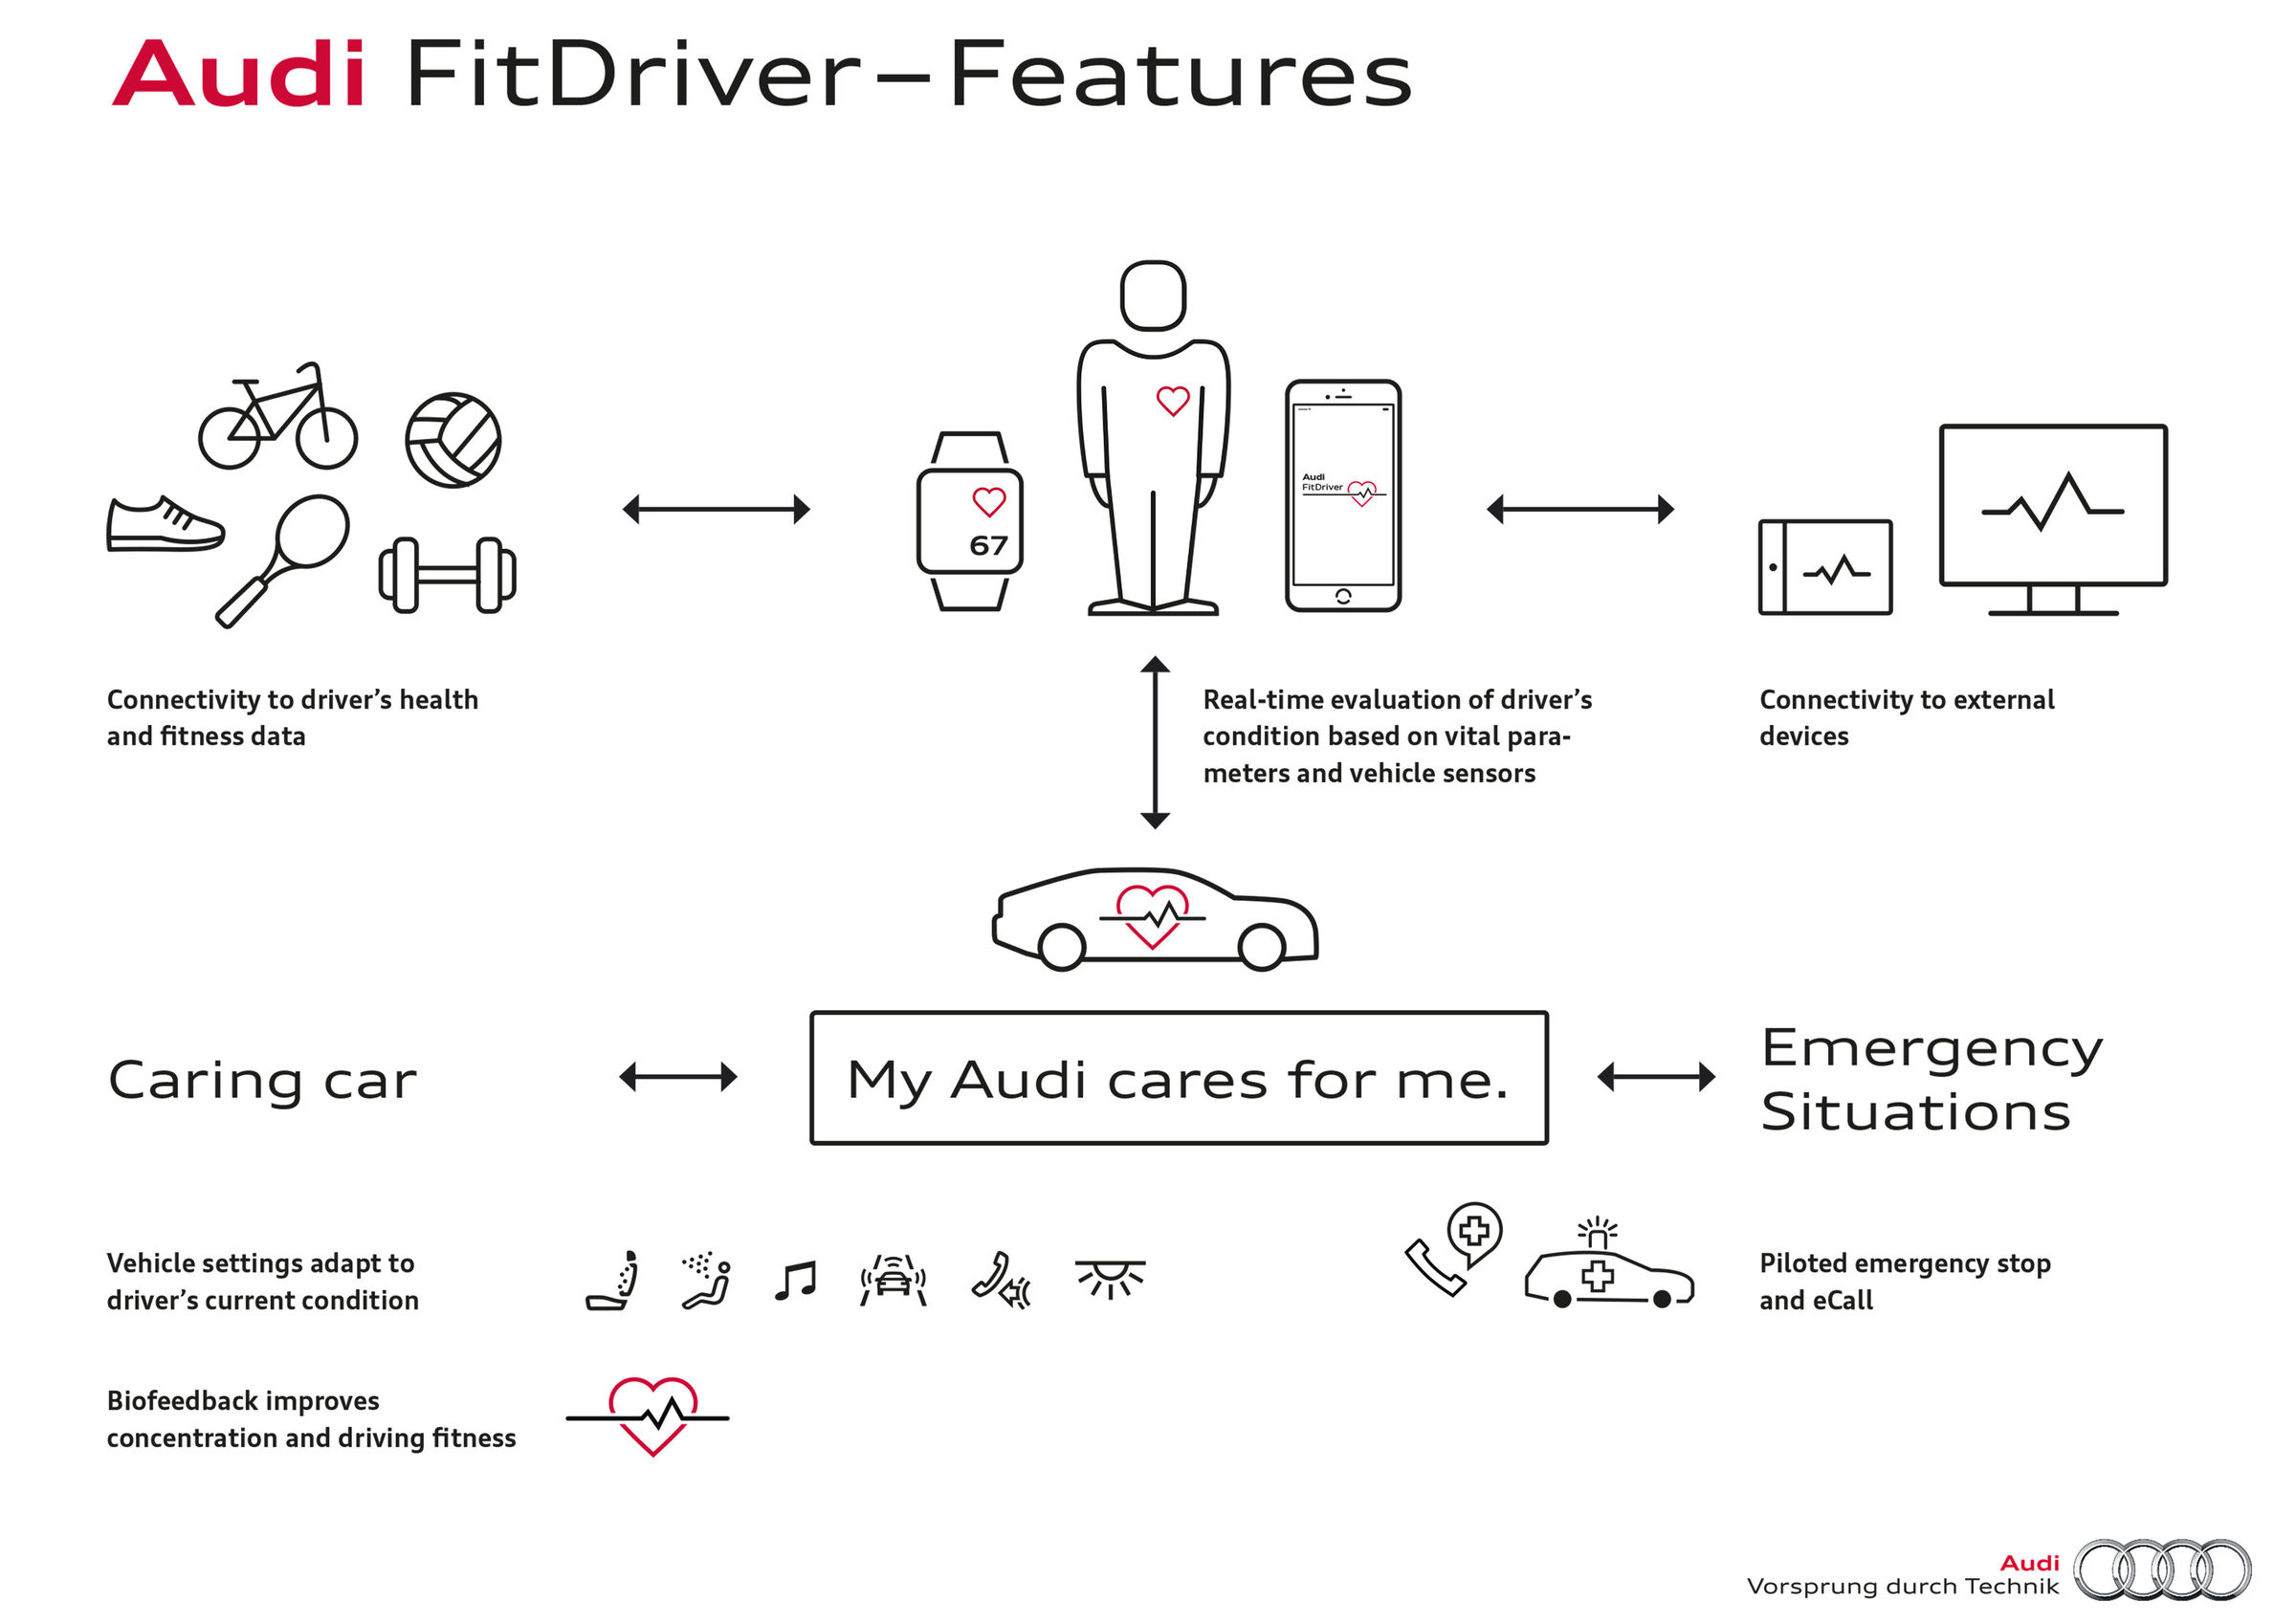
\includegraphics[scale=0.4]{audi_fit_driver} 
\centering
\caption{Model funkcionality komponentov Audi Fit Driver\cite{main}}
\label{fig1}
\end {figure}

Na obrázku ~\ref{fig1} môžeme jasne vidieť, ako prebieha monitorovanie pasažiera v reálnom čase. Môžeme pozorovať, že riešenie danej situácie vyplýva z jej závažnosti. Napriek tomu, že tento projekt vyzerá byť veľmi dobre navrhnutý, sú tu isté faktory ktoré, by mohli viesť k jeho zlyhaniu. Jedným z nich je napríklad výdrž batérie hodiniek, ktorá môže mať za výsledok pozastavenie výmeny informácií medzi servermi a samotným automobilom a preto v prípade rizikovej situácie, nemusia byť softvéry na jej riešenie plne dostupné. Tento problém by sa dal potencionálne odstrániť jednoduchým warningom, ktorý by upozornil vodiča aby si dané zariadenie čo najskôr dobil, aby bolo plne funkčné v prípade rizikových situácií.

\subsection{Pasenger monitoring using AI radar} \label{predstavenie:radar}

Pasenger monitoring system je veľmi dôležitým softvérom, ktorý má za úlohu rozpoznávať živé objekty a ich počet v automobile. Na prvý pohľad sa nám môže zdať zámer tohto softvéru nejasný, no zoberme si veľmi častú situáciu ktorá nastáva najmä v letných mesiacoch. Podľa skupiny Kids and Cars prišlo v automobiloch od roku 1990 až po súčastnosť o život skoro 1000 detí na následky prehriatia organizmu alebo naopak umrznutia.\cite{monitoring} A to nehovoriac ešte o nespočetnom množstve domácich zvierat. Ľudom sa často stáva že v rýchlom okamihu zabudnú svoje dieťa alebo domáce zviera v aute a niekedy stačí naozaj chvíľa a už je neskoro na ich záchranu. Toto je dôvod prečo bol navrhnutý Passenger monitoring system. Budem sa zaoberať druhom systému, ktorý na túto detekciu využíva radar umelej inteligencie. Prečo práve radar? Odpoveď je jasná. Radar na rozdieľ od ultrazvukových senzorov nestráca výkonnosť pri prechode viacerými materiálmi, tým pádom môže byť umiestnený kdekoľvek v automobile a stále mať 100\% výsledok pri zbere dát. Ďalšou možnosťou je aj kamerový systém ktorý by na základe pohybu dokázal zbierať potrebné údaje. Táto možnosť je síce lákavá, ale jej nevýhodou je narúšanie súkromia vlastníka automobilu.

\subsubsection{Presence-Absence Detection Algorithm (PAD)} \label{predstavenie:radar:pad}

Toto je algoritmus bol implementovaný do radaru umelej inteligencie na detekciu živých organizmov v automobiloch. Spočíva na báze machine-learningu a výsledky ktoré prináša musia byť 100\%-tné, pretože akákoľvek malá chyba môže pripraviť niekoho alebo niečo o život. Tento algoritmus nemá za úlohu zisťovať pozíciu a druh organizmov, ale iba rozlíšiť či sa v automobile nachádza živý organizmus. Rozlišuje to na základe najväčšieho rozdielu medzi živým organizom a neživými vecami, dýchacích cyklov. Ak sú niekde v automobile zaznamenané dýchacie cykly, algoritmus okamžite vyšle signál o prítomnosti živého organizmu.\cite{monitoring} Tento algoritmus bol testovaný pri 65 rôznych scenároch a každý z nich trval v priemere viac ako 3 minúty. Radarom bolo zozbieraných okolo 300 minút čistých dát, ktoré algoritmus prešiel a vyhodnotil všetky bez jedinej chyby.

\subsubsection{Passenger Counting Algorithm} \label{predstavenie:radar:pca}

PCA\cite{monitoring} je ďalším algoritmom implementovaným v danom radare ktorý má za úlohu detekovať počet a rozmiestnenie osôb v automobile. Počas testovania bolo zozbieraných 192 minút dát pri 32 možných situáciach. Pri týchto testoch boli použité 3 machine learning algoritmy. Sú to Random Forest (RF), K-Nearest Neighbors (KNN) a Support Vector Machine (SVM). Každý z nich prechádzal zozbieranými dátami a na grafe môžeme vidieť ich konečnú presnosť. A môžeme s istotou povedať, že algoritmus Support Vector Machine priniesol najlepšie výsledky.

\begin {figure} [H]
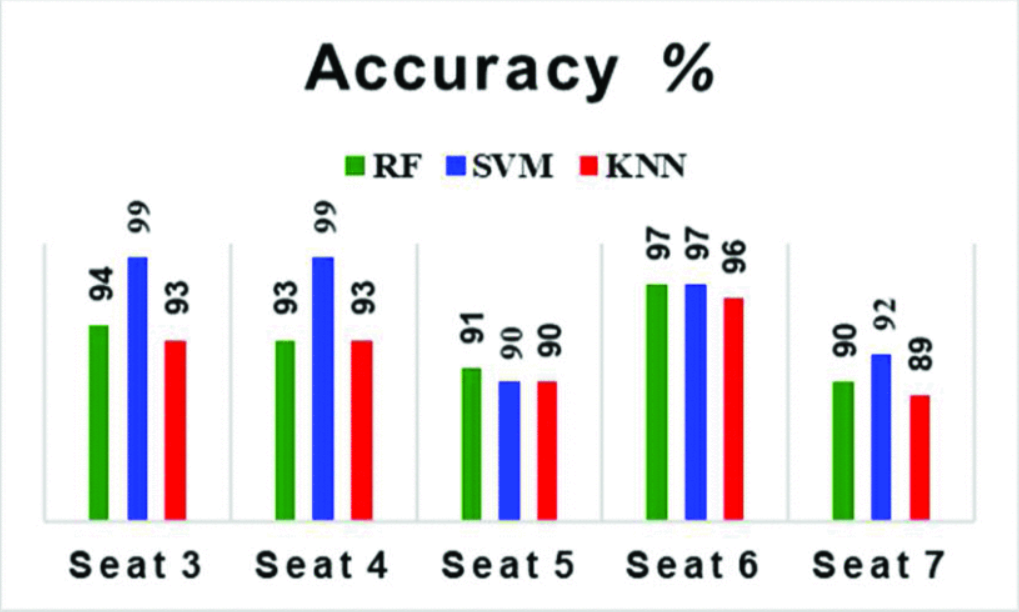
\includegraphics[scale=0.3]{accuracy} 
\centering
\caption{Graf vyobrazujúci presnosť algoritmov pre rôzne sedadlá\cite{monitoring}}
\label{fig1}
\end {figure}

\subsection{Hearth rate monitoring system} \label{predstavenie:hearth}
Low-Cost Real-Time Hearth Rate monitoring system je ďalší softvér, ktorého úlohou je včasne predchádzať veľmi nebezpečným situáciam v doprave. Podobne ako predošlé softvéry, je založený na neustálom monitorovaní vodiča v automobile. Metóda ktorá bola použitá na toto monitorovanie, je implementácia low-cost kamery, ktorá počas jazdy zachytáva tvár vodiča a je napojená na funkciu autopilota a Google/IO.\cite{hearth} 

\subsubsection{Remote Photoplethysmography (rPPG)} \label{predstavenie:heathr:rppg}
Remote Photoplethysmography je metóda ktorá bola použitá na zachytávanie dát z vodičovej tváre. Existuje veľa iných kvalitných spôsobov ako docieliť podobného výsledku, ale veľa z nich je napríklad finančne nákladných alebo náročných na implementáciu v bežných automobiloch a preto ich táto metóda všetky prevyšuje. Jej funkcionalita je založená na extrakcii tepu srdca na základe zmeny zafarbenia pokožky tváre pri každej pulzácii.\cite{hearth} Tieto zafarbenia nie sú pozorovateľné ľudským okom a sú zbierané pomocou odrazu svetla od vodičovej pokožky. Na začiatku tento softvér rozpoznáva či sa pred kamerou nachádza ľudská tvár. Ak áno, začne s meraním. Počas merania zachytáva RGB signály z pokožky vodiča a následne ich pomocou rôznych algoritmov spracuje do dát, ktoré sú ihneď vyhodnocované a na základe výsledku tento softvér zakročí.

\begin {figure} [H]
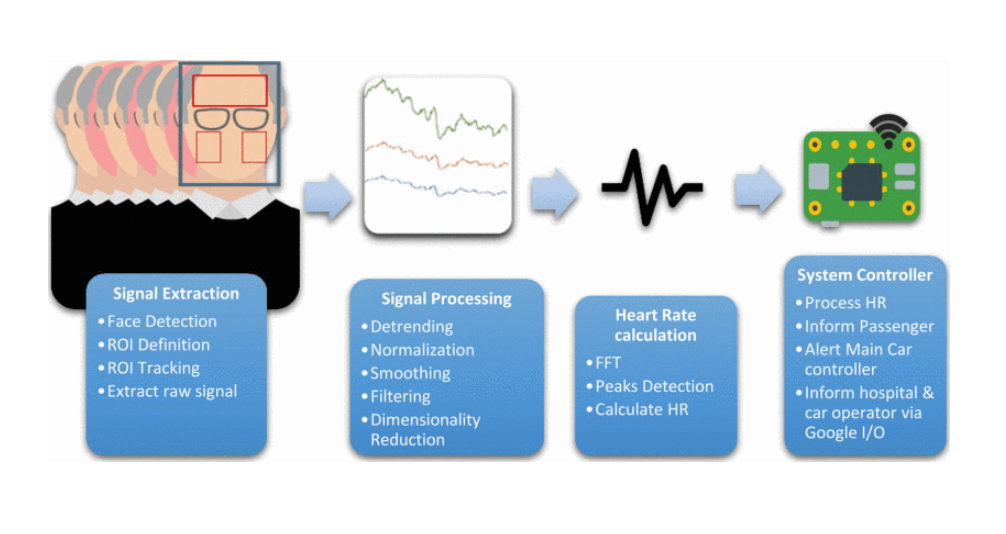
\includegraphics[scale=0.3]{hearth_rate_monitoring} 
\centering
\caption{Reprezentácia spracovávania dát Hearth rate monitoring systémom\cite{hearth}}
\label{fig1}
\end {figure}

\section{Modelovanie situácií} \label{modelovanie}

\begin{figure} [H]

\begin{subfigure}{.5\textwidth}
  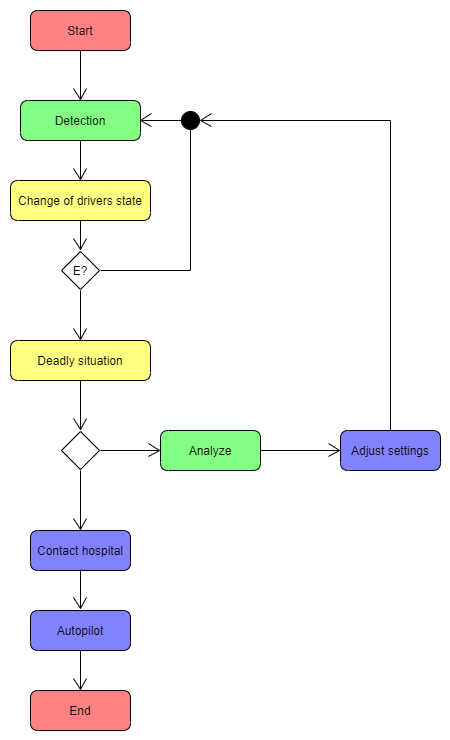
\includegraphics[width=1\linewidth]{EmergencyDiagram}
  \caption{Audi Fit Driver}
  \label{fig:sub1}
\end{subfigure}
\begin{subfigure}{.35\textwidth}
  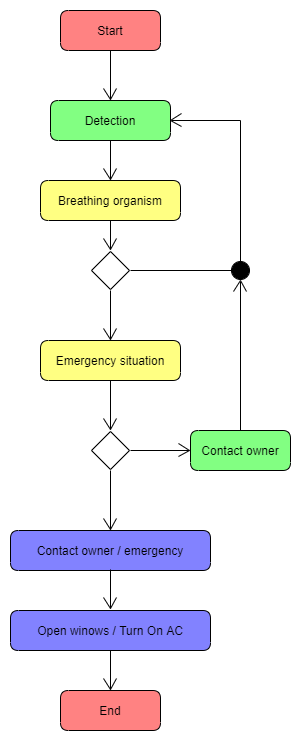
\includegraphics[width=1\linewidth]{AI_Radar}
  \caption{Passenger monitoring}
  \label{fig:sub2}
\end{subfigure}
\caption{Ukážka modelovania situácií jednotlivých softvérov [Author]}
\label{fig:test}
\end{figure}

\section{Osobné zhrnutie jednotlivých tém} \label{zaver} 
\paragraph{Spoločenské súvislosti.}
 \paragraph{Historické súvislosti.}
 \paragraph{Technológia a ľudia.}
\paragraph{Udržateľnosť a etika.}

\section{Záver} \label{zaver} 
%Zhrnutie celeho projektu a moj osobny pohlad na problematiku

\bibliographystyle{plain}
\bibliography{bibliografia.bib}
\end{document}